\documentclass[twoside]{article}
\usepackage{aistats2e}
% \documentclass{article}
% \usepackage{nips12submit_e,times}
\usepackage{tikz}
\tikzstyle{vertex}=[auto=left,circle,fill=black!25,minimum size=20pt,inner sep=0pt]
\usepackage{verbatim}
\usepackage{url}
\usepackage{graphicx, color}
\usepackage{amsmath}
\usepackage{caption}
\usepackage{subcaption}
\usepackage{footnote}
\usepackage{sidecap}
\DeclareCaptionType{copyrightbox}

%\usepackage[accepted]{aistats2e}

\begin{document}

\twocolumn[

\aistatstitle{Stochastic blockmodeling of relational event dynamics}

\aistatsauthor{ Anonymous Author 1 \And Anonymous Author 2 \And Anonymous Author 3 }

\aistatsaddress{ Unknown Institution 1 \And Unknown Institution 2 \And Unknown Institution 3 } ]

%\maketitle
\begin{abstract}
%Observing network data as a sequence of relational events provides an opportunity to understand differences in how individuals interact over time.
For continuous-time network data, several approaches have recently been proposed for modeling dyadic event rates conditioned on the observed history of events and nodal or dyadic covariates.  In many cases, however, interaction propensities -- and even the underlying mechanisms of interaction -- vary systematically across subgroups whose identities are unobserved.
For static networks, such heterogeneity has been treated via methods such as stochastic blockmodeling, which operate by assuming latent groups of individuals with similar tendencies in their group-wise interactions.
Here, we combine these two approaches by positing a latent partition of the node set such that event dynamics within and between subsets evolve in potentially distinct ways.
We illustrate the use of our model family by application to several forms of dyadic interaction data, including email communication and Twitter direct messages.
Parameter estimates from the fitted models clearly reveal heterogeneity in the dynamics among groups of individuals.
We also find that the fitted models have better predictive accuracy than either baseline models or relational event models without latent structure.
Our approach illustrates the utility of latent structure methods based on detailed dynamics, which can succeed even in the absence of differences in marginal interaction rates across groups. 
%{ \color{red}  TODO: This last sentence is a bit unclear for a new reader. TODO: A few of theses sentences might be too long. TODO: stream vs sequence in first sentence?}
\end{abstract}

\section{Introduction}

Statistical methods for analyzing network data are becoming increasingly useful for studying phenomena ranging from online social behavior to protein  interactions \cite{Goldenberg2009}.
Recent work has expanded to include settings in which we observe events occurring between nodes over time (i.e., \emph{relational events}, as opposed to static edge structures or ongoing relationships), with the common goal of modeling interaction dynamics in terms of both endogenous mechanisms and exogenous covariates.  
A key concern in this regard is the ability to detect differential behavioral tendencies on the part of subsets of nodes, the dynamic analog of \emph{role structure} in classical network analysis \cite{Wasserman1994}.  

In the cross-sectional case, \emph{stochastic blockmodels} \cite{Nowicki2001} have been proposed as a family of approaches that capture behavioral similarity by identifying subsets of nodes with similar patterns of ties to those in other sets.  While it is natural to apply these ideas directly to relational event data via blockmodeling of the time-marginalized rates of interaction among dyads (effectively treating the event structure as a valued graph), there are limits to what this approach can detect.  Consider, e.g., Figure~\ref{fig:introexample}.  In the top left panel, we depict the time-marginalized frequencies of simulated interactions between members of two groups (A and B), with darker cells indicating higher interaction frequencies.  As can be seen, a clear role structure is present, with members of each subgroup interacting at higher rates with co-members than out-group members; such a structure is easily detectable via conventional blockmodeling techniques.  By contrast, consider the interaction patterns shown in the top right panel.  Here, there is no systematic difference in marginal rates between the two groups, rendering them invisible under a standard blockmodeling approach.

There is, however, a difference to be detected.  The bottom panels of Figure~\ref{fig:introexample} show, for each respective simulation, parameters (as discussed in Section~\ref{sec:specification}) governing the tendency towards reciprocation for members of each group vis a vis communications coming from in- or out-group members.  For both simulated cases, the log-hazard for an event in which a member of group A or group B immediately responds to an incoming communication from an in-group member is increased by an increment of 2 (relative to a non-reciprocating event), and the log-hazard for an event in which a member of group B immediately responds to an incoming communication from a member of group A is increased by a corresponding increment of 0.5.  Groups A and B are thus distinctive in terms of their dynamic behavior, even in the absence of marginal differences in propensity to communicate.  A blockmodeling approach that classifies nodes based on shared dynamics (rather than merely shared marginal communication rates) can potentially identify such subtle distinctions; in this paper, we introduce such an approach.


%For example, a common aspect of human communication is \emph{reciprocity}: person A speaks to person B, then B has a higher propensity to speak to A.  
%Through an event-based analysis we can study how nodes vary in their tendencies to behave in this manner.  %the similarity --- and differences --- in the dynamics of nodes in the network. 
%This is particularly relevant when studying interactions among students in a classroom, where differences in conversational tendencies might be associated with covariates about the student or classroom, or based on unobserved groupings, and may have ramifications for education.
%In such contexts, a standard blockmodel only provides a means for studying the structure of marginal rates of communication, but not the shared tendencies in the dynamics of the sequence of events.

%When such .  One unifying idea is that the nodes of these networks are differentiated by rates of interacting with other parts of the network [TODO], where this variation in rates may be associated with some unobserved quantity, e.g. a covariate such as age or sex, or perhaps shared [TODO].
%Stochastic blockmodels \cite{Nowicki2001, Kemp, Ishiguro2010, Rodriguez} are a class of statistical models for static network data that employ latent variables to model this heterogeneity by .  Such techniques are readily applied to count data, [TODO: These let us study how shared behavior is associated with other covariates.]

%1) assuming each node in the network belongs to some block (or cluster) and 2) parameterizing the probability of a tie between members

%PS: much of this past work is for static network data. Do we want to make the observation here that we are thinking about blockmodels for *rate* data here in our discussion and in our example in figure 1 - if we don't some readers/reviewers might get a little confused. For example we could say that instead of a binomial model on edges we can think of a Poisson process yielding counts over time, where we can still think about blockmodels. 
%PS: also, we introduce the term "rates" above without really defining it, and then go on to talk about "mean rate" below. So I think we definitely need a sentence somewhere above that makes it clear we are talking about edges that instantaneously appear and disappear over time at some rate, rather than static edges.

%If we are interested in studying a network of events, there are other important aspects of the dynamics in addition to the mean rate. 
%For example, human conversation often has an increased propensity for reciprocated events.
%PS: wording of next sentence is a little odd - not sure I understand what it means...
%Shared tendencies based on other observed or unobserved quantities is of interest (who shares this tendency).
%[TODO: Example of a shared dynamic... perhaps sticking with the reciprocity bit.]
%Figure \ref{fig:introexample} shows a simple example of how traditional blockmodels are unable to make inferences these types of dynamic phenomena. 


%A limitation of all of these approaches is the assumption of a single common behavior for all individuals.
%In contrast, in real-world networks it is reasonable to expect {\it heterogeneity} in dynamic behavior.  
%In an organization, the manner in which an individual communicates with others may be a function of an individual's {\it role} in the organization.
%For example, in a university,  email communication patterns over time between professors, students, and staff will likely be quite different within and between the three groups.

% - used to thinking about actors differentiated by rates
% - other things in the dynamics than rates, e.g. form of interaction.
% - Also important aspect of modeling social dynamics.
% especially important in cases like plot 1(c) where classical methods
% will fail.

%PS: not totally happy with this example since the "roles" are completely determined by one's "job title" and I think we would prefer something
% less explicit, e.g., that there are "leaders", "followers", etc, that go beyond just job titles. So feel free to edit this further!

%
%comprised of several teams, each team may uncover different patterns for collaborating via email---individuals in one group may respond more quickly, while another group may preferentially send to highly active individuals.

Borrowing from the intuition of stochastic blockmodels, we propose a novel continuous-time model family for network-based event sequences where latent clusters of nodes share similar patterns of interaction.
Our approach employs a flexible framework for  specifying how the process depends on the previous history of events \cite{AalenOddO.2008, Butts2008}.
In this way one can compare theories about underlying processes and make predictions about future data conditioned on the past, simultaneously adjusting for unobserved heterogeneity.

We describe how we learn the latent cluster assignments and model parameters via MCMC, and illustrate the behavior of the model with simulated data.
Using several real-world social network data sets involving dyadic communication, we compare the predictive performance of the fitted models to standard baselines.
We conclude by showing that the parameter estimates reveal interpretable structure in the event dynamics, enabling the study of a dynamic extension to stochastic equivalence.

\begin{figure}
\centering
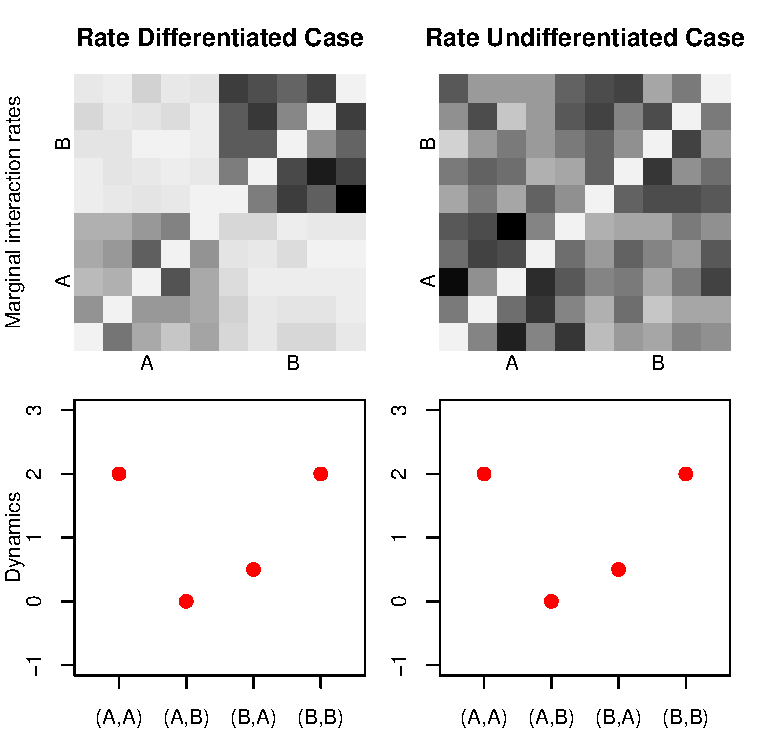
\includegraphics[scale=.5]{../figs/introexample/all}
\caption{Illustration of differentiation by rate of interaction versus by dynamic behavior.  The left column shows an example where within-block communication is large, and there is a higher tendency for reciprocity within a block.  In the situation where the two groups are not differentiated by rate, as in the right column, a standard blockmodel is unable to distinguish between groups A and B.  The proposed method can, however, learn such groups by employing more flexible definitions of shared dynamics.}
\label{fig:introexample}
\end{figure}
% {\color{red} (Suggest renaming "Dynamics parameters" to "Behavioral parameters" or something.  "Dynamics parameters" is not gramatically sound.)

\section{Model}

Consider a sequence of events $\mathcal{A} = (0,t_1, \ldots, t_M)$ arising from a nonhomogeneous Poisson process with  intensity $\lambda(t)$.
If the intensity is left continuous and piecewise constant with respect to a set of knots $\tau$ then the likelihood can be written
\begin{align}
\mathcal{L}(\mathcal{A}|\theta) &= \prod_{m=1}^M \lambda(t_m) \exp\left\{ - \int_{0}^{t_M} \lambda(s)ds \right\} \notag  \\
&= \prod_{m=1}^M \lambda(t_m) \prod_{k=1}^{|\tau|} \exp\left\{ - (\tau_{k} - \tau_{k-1}) \lambda(\tau_k) \right\}%  \exp\left\{ - (t - \tau_{M}) \lambda(t) \right\}
\end{align}
%{\color{red} (You've left out the right-censoring factor here (and also below).)}

One can extend the above to marked point processes where each event contains additional information.  {\color{red} In Figure \ref{fig:example}a we illustrate the case of \emph{relational events}  occurring among $N$ nodes}, where each event in the process contains both a sender $i$ and a recipient $j$ such that  $(i,j) \in \mathcal{R}$, where $\mathcal{R}$ is the \emph{risk set} is defined as the set of all possible dyadic events.
{\color{red} The study of human communication often involves such data (e.g. phone calls, online interaction, etc.) where the nodes represent people and each event represents one person speaking to another.}

As in \cite{Butts} in the proposed approach we assume each event involving dyad $(i,j) \in \mathcal{R}$ occurs as a Poisson process with intensity $\lambda_{i,j}(t|\cdot)$ that is piecewise constant and depends on the previous history of events  $\mathcal{A}_t = \{(t_m,i_m,j_m): t_m \in [0,t) \}$.  
%The likelihood of an observed event history $\mathcal{A}$ extending from time 0 to the time of the final event, $t_M$, is 
The likelihood of an observed event history $\mathcal{A}_{t_M}$ (extending from time 0 to the time of the final event and denoted $\mathcal{A}$ for convenience) is
%The likelihood of an observed event history $\mathcal{A}_{t_M}$ (also denoted $\mathcal{A}$ for convenience) is
\begin{align}
\mathcal{L}(\mathcal{A}|\theta) &= \prod_{m=1}^M \lambda_{i_m,j_m}(t_m|\cdot) \prod_{(i,j) \in \mathcal{R}}\exp\{ - (t_m - t_{m-1}) \lambda_{i,j}(t_m | \cdot) \}
\label{eqn:llk}
\end{align}

\begin{figure*}
\begin{subfigure}[b]{0.45\linewidth}
\centering
  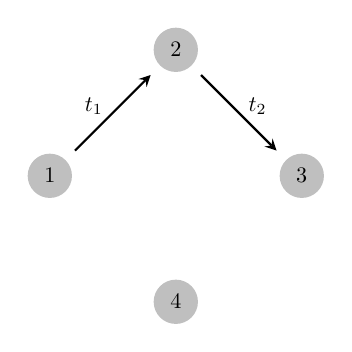
\begin{tikzpicture}[scale=.8,transform shape,thick]
    \node[vertex] (n1) at (0,0)  {1};
    \node[vertex] (n2) at (2,2)  {2};
    \node[vertex] (n3) at (4,0) {3};
    \node[vertex] (n4) at (2,-2) {4};
    \draw[-stealth] (.4,.4) -- (1.6,1.6);
    \draw[-stealth] (2.4,1.6) -- (3.6,.4);
    \node at (.7,1.1) {$t_1$};
    \node at (3.3,1.1) {$t_2$};
  \end{tikzpicture}
  \caption{Dynamic network data}
\end{subfigure}
\begin{subfigure}[b]{0.45\linewidth}
\centering
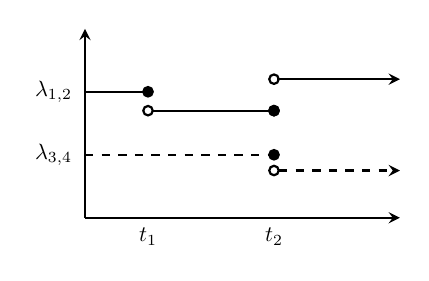
\begin{tikzpicture}[scale=.8,transform shape,thick]
\draw[-stealth] (0,0) -- (0,3);
\draw[-stealth] (0,0) -- (5,0);

% First timeline
\draw (0,2) -- (1,2);
\draw[fill=black] (1,2) circle (0.75mm);
\draw (1,1.7) circle (0.75mm);
\draw (1.08,1.7) -- (3,1.7);
\draw[fill=black] (3,1.7) circle (0.75mm);
\draw (3,1.7) circle (0.75mm);
\draw (3,2.2) circle (0.75mm);
\draw[-stealth] (3.05,2.2) -- (5,2.2);

% second timeline
\draw[dashed] (0,1) -- (3,1);
\draw[fill=black] (3,1) circle (0.75mm);
\draw (3,.75) circle (0.75mm);
\draw[dashed, -stealth] (3.08,.75) -- (5,.75);

% labels
\node at (-.5,2) {$\lambda_{1,2}$};
\node at (-.5,1) {$\lambda_{3,4}$};
\node at (1,-.3) {$t_1$};
\node at (3,-.3) {$t_2$};
\end{tikzpicture}
\caption{Intensities for two dyads}
\end{subfigure}
\caption[]{Illustration of relational event data and the assumptions of the model.  (a) A sequence of two events among four nodes: (1,2) occurs at time $t_1$ and (2,3) occurs at time $t_2$. (b) The intensity functions $\lambda_{1,2}(t)$ (solid) and $\lambda_{3,4}(t)$ (dashed).  We assume $\lambda_{3,4}(t)$ can only change after events sent or received by node 3. }
\label{fig:example}
\end{figure*}

Here, we aim to learn about the dynamics within and between subsets of nodes.   To facilitate this, we propose a novel extension which assumes each node $i$ belongs to latent cluster $z_i$ while still using a log linear model for the intensity functions
\begin{align*}
\log \lambda_{i,j}(t | \mathcal{A}_t,\mathbf{\beta},\mathbf{z}) &= \boldsymbol{\beta}'_{z_i,z_j} \mathbf{s}(t,i,j,\mathcal{A}_t)
%z_i &\sim \mbox{CRP}(\alpha) &
%\boldsymbol{\beta}_{k,l} &\sim %\mbox{N}_p(\boldsymbol{\mu},\boldsymbol{\sigma}^2I)
\end{align*}
where for each pair of clusters $(k,l)$ we have a parameter vector $\boldsymbol{\beta}_{k,l} \sim \mbox{Normal}(\boldsymbol{\mu},\boldsymbol{\sigma}^2I)$ that corresponds to the $P$-dimensional vector of statistics $\mathbf{s}(t,i,j,\mathcal{A}_t)$ computed from the previous history $\mathcal{A}_t$.
Thus, the rate of $(i,j)$ events has the same parameters as other events occurring between group $z_i$ and $z_j$.

% In practice we may believe an interaction between one dyad should not affect the rate of an entirely separate dyad.
As shown in Figure \ref{fig:example}, we only allow each intensity function $\lambda_{i,j}(t)$ to change following an event where $i$ was the sender or the recipient.
This is sensible in distributed settings where $i$ has limited knowledge about interactions among other actors.
% In the Supplementary Material we show how this assumption also reduces the computational complexity of computing the above likelihood.

We allow the blocks to share information by placing a hierarchical prior on the collection of $\boldsymbol{\beta}_{k.l}$ where $\mu_p \propto N(0,1)$ and $\sigma_p^2 \sim \mbox{Inv-Gamma}(\alpha_{\sigma},\beta_{\sigma})$.
The cluster assignments are given a non-parameteric prior $z_i \sim \mbox{CRP}(\alpha)$, allowing for a flexible number of clusters.
% TODO: expand on this

\subsection{Model specification}
\label{sec:specification}


Table ~\ref{tab:stats}  lists the statistics  $\mathbf{s}(t,i,j,\mathcal{A}_t)$ used in Section \ref{sec:experiments}.
For example, a particular node sending often may indicate they will continue to be a sender in the future.
We use $\mathbf{I}$ to denote the indicator function where $\mathbf{I}(A) = 1$ if $A$ is true, and 0 otherwise.
We normalize these counts by the number of events up until a dyad's prior changepoint by using $f(x) = \log \frac{x+1}{m + N(N-1)}$. %\footnote{This seems to avoid ``explosion'' when simulating from the model.  TODO: Explore the theory about these sorts of statistics.  Aalen has a few suggestions.}
Other statistics could be of interest for particular substantive questions \cite{Butts2008,Vu2011}.  

The next set of statistics aim to capture various types of \emph{participation shift} that play a role conversational norms \cite{Gibson2003}.
For example, an \texttt{ab-ba} effect indicates an increased propensity for reciprocity where the event $(a,b)$ is followed by $(b,a)$.
{\color{red} Another example is a \emph{turn-taking} effect where an event $(a,b)$ is followed by $b$ initiating an event with an individual other than $a$, denoted \texttt{ab-by}.
These statistics are binary and simply indicate whether or not the event in question can be classified as an example of that particular transition. }
Though only the statistics in Table \ref{tab:stats} are used in our experiments, one may use any quantity that is computed using the previous history of events or known covariates about nodes or dyads.
The only restriction within the proposed framework is that the statistic may not change in value between each observed event.%\footnote{This prevents one from using the number of events occurring in some previous time window, as in \cite{Gunawardana2011}.}
% TODO: Also, need to be restricted to ego conditions if we want it fast

\subsection{Relation to other models}

Our formulation is reminiscent of the stochastic blockmodel \cite{Nowicki2001} for static networks which models the probability of a dyad as $p(y_{i,j}) =\mbox{logit}^{-1}( \eta_{z_i,z_j})$ where $\eta_{z_i,z_j}$ is interpreted as a mixing rate between group $z_i$ and group $z_j$.
In the proposed method, however, the blockmodel structure facilitates the study of intra-group and inter-group dynamics via a continuous-time network model.

The proposed family of models generalizes several important special cases.
For example,  using only the intercept statistic $s_0(t,i,j,\mathcal{A}_t) = 1$ is analogous to the stochastic block model for static networks.
Under this model each dyad is a homogeneous Poisson process and all dyad intensities $\lambda_{i,j}$ within block $(z_i,z_j)$ have the same intensity, $\exp\{\boldsymbol{\beta}_{z_i,z_j}\}$.
As these intensities do not change under this specification, the likelihood simplifies to
\begin{align}
\mathcal{L}(\mathcal{A}|\beta) = \prod_{m=1}^M \lambda_{i_m,j_m}
\prod_{(i,j) \in \mathcal{R}} \exp\{-t_M \lambda_{i,j}\}
\end{align}
Alternatively, if one models only the order of the events (ignoring the times at which they occur), the likelihood can be written as
\begin{align}
\mathcal{L}_{\mbox{mult}}(\mathcal{A}|\beta) = \prod_{m=1}^M \frac{\lambda_{i_m,j_m}(t_m | \cdot)}{\sum_{(i,j) \in \mathcal{R}} \lambda_{i,j}(t_m | \cdot)}.
\label{eqn:multllk}
\end{align}
The functional form is similar to conditional logit models used for discrete choice data \cite{McFadden1973}, though here the possible choices are all the dyads in $\mathcal{R}$.

\begin{table*}[t]
\footnotesize
\center
\begin{tabular}{|l|l|}
\hline
Statistic & Formula\\
\hline
\hline
Intercept& $s_{0}(t,i,j,\mathcal{A}_t) = 1$\\
Reciprocity (AB-BA)& $s_{1}(t,i,j,\mathcal{A}_t) = \mathbf{I}(i_m=i,j_m=j,i_{v_{mij}}=j,j_{v_{mij}}=i)$\\
Turn-continuing (AB-AY)& $s_{2}(t,i,j,\mathcal{A}_t) =  \mathbf{I}(i_m=i,j_m=j,i_{v_{mij}}=i,j_{v_{mij}}\ne j)$\\
Turn-taking (AB-BY)&$s_{3}(t,i,j,\mathcal{A}_t) = \mathbf{I}(i_m=i,j_m=j,i_{v_{mij}}=j,j_{v_{mij}}\ne i)$\\
%Turn-usurping (AB-XA)& $s_{7}(t,i,j) = \mathbf{I}(i_m=i,j_m=j,i_{v_{mij}} \ne j,j_{v_{mij}}=i)$\\
%Turn-usurping (AB-XB)&$s_{8}(t,i,j) = \mathbf{I}(i_m=i,j_m=j,i_{v_{mij}} \ne i,j_{v_{mij}}=j)$\\
Sender out-degree& $s_{4}(t,i,j,\mathcal{A}_t) = f(\sum_{m:t_m<t} \mathbf{I}(i_m=i) )$\\
Sender in-degree& $s_{5}(t,i,j,\mathcal{A}_t) = f(\sum_{m:t_m<t} \mathbf{I}(j_m=i) )$\\
Dyad count& $s_{6}(t,i,j,\mathcal{A}_t) = f(\sum_{m:t_m<t} \mathbf{I}(i_m=i,j_m=j) )$\\
%Receiver out-degree& $s_{3}(t,i,j) = f(\sum_{m:t_m<t} \mathbf{I}(i_m=j))$\\
%Receiver in-degree& $s_{4}(t,i,j) = f(\sum_{m:t_m<t} \mathbf{I}(j_m=j))$\\
\hline
\end{tabular}
\caption{Statistics used to specify intensity functions using the previous history $\mathcal{A}_t$, where $v_{mij}$ is the index of the changepoint for $\lambda_{i,j}(t)$ previous to event $m$. }
\label{tab:stats}
\end{table*}

\subsection{Related work}
Stochastic blockmodels have been extended to longitudinal network data
involving a sequence of networks occurring at discrete times
\cite{Ishiguro2010, Rodriguez2011}, while we focus on methods for
analyzing a stream of relational events. 
The proposed model is an extension of recent work on modeling event-based social network data using an event history approach \cite{Butts2008,Brandes2009,Perry2011,Stadtfeld2011,Vu2011,Vu2011a}. % \cite{AalenOddO.2008} Opsahl2011,Stadtfeld2010
Relational event models such as these require a knot at each observed event, while other approaches such as \cite{Gunawardana2011} learn the regions where an intensity is constant.
By using decision trees,  \cite{Gunawardana2011} also allow for a nonlinear relationship between statistics and intensity functions.  
We instead use latent variables to allow for heterogeneity in intensities across the set of possible events.


\section{Inference}

We use Markov chain Monte Carlo to sample from the posterior distribution of our parameters.%\footnote{TODO: Describe why EM is hard.} % Note that approaches such as EM are difficult since the form of the likelihood does not admit an analytic expression for the expected complete data log likelihood.

\subsection{Sampling $\mathbf{z}$ given $\boldsymbol{\beta}$ and $\mathcal{A}$ }

We use Gibbs sampling to sample the latent class assignments $\mathbf{z}$ from the conditional distribution
\begin{align*}
p(z_r | \mathbf{z}_{-r},\mathcal{A},\alpha,\boldsymbol{\beta}) \propto&  p(\mathcal{A}|\mathbf{z},\boldsymbol{\beta}) p(z_r | \mathbf{z}_{-r},\alpha) \\
p(\mathcal{A}|\mathbf{z},\boldsymbol{\beta}) \propto &
\prod_{m=1}^M \lambda_{i_m,j_m}(t_m|\cdot)^{\mathbf{1}[r \in \{i_m,j_m\}]} \ \   \times \\
&\prod_{(i,j) \in \mathcal{U}_r} \exp \{ -(t_m - t_{m-1}) \lambda_{i,j}(t_m|\cdot)\}
\end{align*}
where $\mathcal{U}_r = \{(i,j) \in \mathcal{R}: r \in \{i,j\}\}$ is the set of dyads involving node $r$.
Under a CRP($\alpha$) prior, we have $p(z_i = k | z_{-i},\alpha) = n_k $ and $p(z_i = K+1 |  z_{-i},\alpha) = \alpha$ where $n_k$ is the number of nodes assigned to cluster $k$.

\subsection{Sampling $\boldsymbol{\beta}$ given $\mathbf{z}$ and $\mathcal{A}$ }

For each block $(k,l)$ we need to sample the vector of parameters $\boldsymbol{\beta}_{k,l}$ from its posterior
\begin{align*}
p(\boldsymbol{\beta}_{k,l} | \mathcal{A}, \textbf{z}, \boldsymbol{\mu}, \boldsymbol{\sigma}) &\propto p(\boldsymbol{\beta}_{k,l} | \boldsymbol{\mu}, \boldsymbol{\sigma}) p( \mathcal{A}| \textbf{z}, \boldsymbol{\beta}) \\
p(\boldsymbol{\beta}_{k,l} | \mu, \sigma) &= \prod_{p=1}^Pp(\beta_{k,l,p}|\mu_p,\sigma_p^2)\\
p(\mathcal{A}|\mathbf{z},\boldsymbol{\beta}) &\propto \prod_{m=1}^M \lambda_{i_m,j_m}(t_m|\cdot)^{\mathbf{1}[(i_m,j_m) \in \mathcal{V}_{k,l}]} \ \times \\
& \ \ \prod_{(i,j) \in \mathcal{V}_{k,l}} \exp \{ -(t_m - t_{m-1}) \lambda_{i,j}(t_m|\cdot)\}
\end{align*}
where $\mathcal{V}_{k,l} = \{(i,j): z_{i} \in \{k,l\} \ \mbox{or} \ z_{j} \in \{k,l\} \}$ is the set of dyads with a sender in group $k$ and a recipient in $l$.  We sample each $\beta_{k,l,p}$ via slice sampling.

\subsection{Sampling $\mu$  and $\sigma$ given $\beta$ }

The inverse gamma distribution is a conjugate prior to a Gaussian distribution with known location parameter, thus $\sigma$ can be sampled from the conditional distribution
\begin{align}
\label{eqn:gibbs.sigma}
\sigma_p^2 &| \boldsymbol{\beta}, \mu_p,  \alpha_{\sigma}, \beta_{\sigma} \sim \\
& \mbox{Inv-Gamma}\left(\alpha_{\sigma} + \frac{K^2}{2}, \beta_{\sigma} + \frac{1}{2} \sum_{k=1}^K\sum_{l=1}^K (\beta_{k,l,p} - \mu_p)^2\right).
\end{align}
Each parameter $\mu_p$ can be sampled from its conditional distribution given $\sigma_p^2$ and the parameters $\boldsymbol{\beta}$,
\begin{align}
\label{eqn:gibbs.mu}
\mu_p | \boldsymbol{\beta},\sigma_p^2 &\sim \mbox{Normal}\left(\frac{1}{K^2}\sum_{k=1}^K \sum_{l=1}^K \beta_{k,l,p},\frac{ \sigma_p^2}{\sqrt{K^2}}\right).
\end{align}

\subsection{Hyperparameter settings}
In our experiments we use $\alpha=1$ and use Algorithm 8 from \cite{Neal2000} with 5 extra clusters drawn from the prior.%\footnote{I also tried out a prior for cluster sizes such that $n_k \sim \mbox{NegBinom}(3,N/K)$, where $K$ is chosen a priori.  This aims for similarly sized groups.}
We set $\alpha_{\sigma}=5$ and $\beta_{\sigma}=1$ so that in the presence of little data we encourage shrinkage towards the upper level parameters $\mu$.  
As with other models, we note that the predictive accuracy of the model can depend on the hyperparameters.

\subsection{Scalability}

Likelihood computation essentially depends on the number of changepoints (i.e. knots) in all of the intensity functions being modeled.   
We take advantage of our restriction on the types of statistics $\mathbf{s}$ to reduce the computational complexity of computing our likelihood  as
\begin{align*}
\mathcal{L}(\mathcal{A}_{t_M}|\theta) &= \prod_{m=1}^M \lambda_{i_m,j_m}(t_m|\cdot) \times \\
&  \prod_{(i,j) \in \mathcal{R}_{i_m,j_m}}\exp\{ - (t_m - \tau_{m,i,j}) \lambda_{i,j}(t_m | \cdot) \}
\end{align*}
\noindent where event $m$ is the dyad $(i_m,j_m)$, $\tau_{m,i,j}$ is the time  of the changepoint for $\lambda_{i,j}(t|\cdot)$ prior to the $m$th event, and $\mathcal{R}_{i,j}$ is the set of dyads whose intensity changes if $(i,j)$ occurs.%  \cite{Butts2008}. %\footnote{We further assume 1) all intensity functions change at times $t=0$ and $t=t_M$, and 2) the first event is drawn uniformly from the risk set.}

 By limiting the number changepoints, computing the likelihood  $p(\mathcal{A}|\mathbf{z},\boldsymbol{\beta})$ for Gibbs sampling $z_r$ is $O(|\mathcal{U}_r| \cdot P \cdot N)$, avoiding a factor of $N^2$.  In practice, we precompute $\tau_{m,i,j}$ and $\mathbf{s}(t_m,i,j,\mathcal{A}_t)$ for all $m$, $i$, and $j$.  This can be done in one pass through the data set.

% The Supplementary Material mentions one attempt at speeding this up, for larger graphs, but additional assumptions/approximations are likely needed for scalability.

\begin{figure*}
%\centering
\begin{subfigure}[b]{0.25\textwidth}
\centering
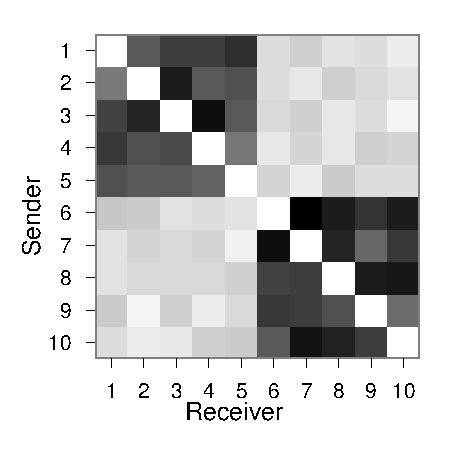
\includegraphics[width=1.8in]{../figs/synthetic/mat.pdf} %counts2.pdf
\vspace{.25cm}
\caption{}
\end{subfigure}
~
\begin{subfigure}[b]{0.3\textwidth}
\centering
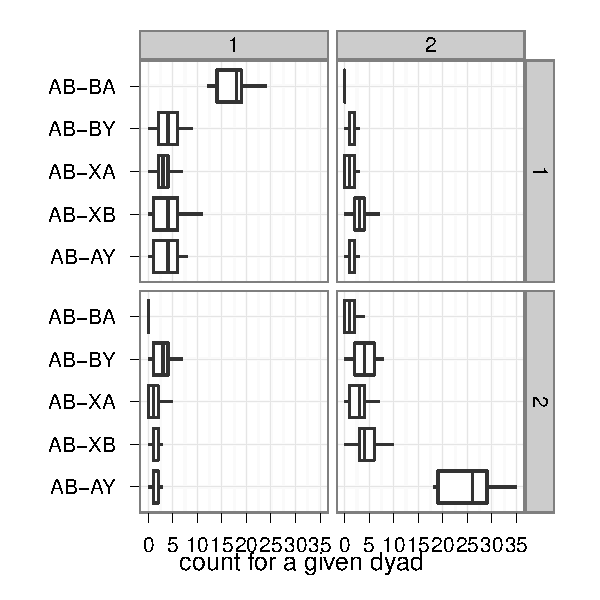
\includegraphics[width=2.4in]{../figs/synthetic/counts.pdf}
\caption{}
\end{subfigure}
~
\begin{subfigure}[b]{0.3\textwidth}
\centering
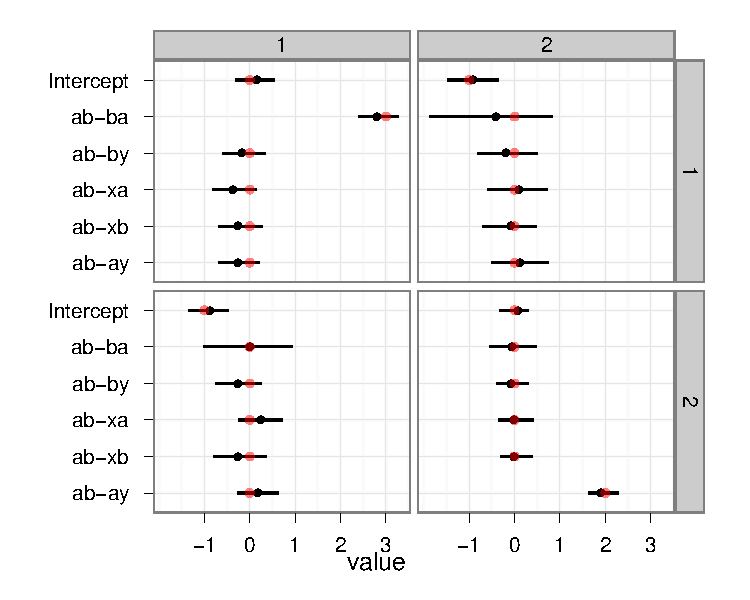
\includegraphics[width=2.5in]{../figs/synthetic/params-estimates.pdf}
\vspace{-.5cm}
\caption{}
\end{subfigure}
\caption{Illustration of 2000 simulated events, as described in text. (a) Counts of each dyad. (b) Boxplot of distribution of participation counts across dyads.  The top left shows an increased propensity for reciprocity within cluster 1; bottom right shows more AB-AY events within cluster 2.  (c) Parameters (in red) and posterior credible intervals (in black).}
\label{fig:syncounts}
\end{figure*}

\section{Simulation}
\label{sec:simulation}

We check our model fitting procedure using a small synthetic data set involving 10 nodes from 2 groups where 1) within group communication is more likely, 2) events among members in the first group are more likely to be reciprocated  (i.e. a positive \texttt{ab-ba} effect), and 3) events among members of the second group are more likely to be followed by an event with the same sender (i.e. a positive \texttt{ab-ay} effect).  The specification of $\textbf{s}$ is therefore $\textbf{s}(t,i,j,\mathcal{A}_t) = [s_0, s_{1}(t,i,j,\mathcal{A}_t), s_{2}(t,i,j,\mathcal{A}_t)]$.  For the synthetic data set we use parameter vectors $\boldsymbol{\beta}_{1,1} = (0,3,0)$,  $\boldsymbol{\beta}_{1,2} = \boldsymbol{\beta}_{2,1} = (-1,0,0)$, and $\boldsymbol{\beta}_{2,2} = (0,2,0)$.
Data is generated by sequentially computing $\lambda_{i,j}(t_m|\cdot)$ for all $(i,j) \in \mathcal{R}$, drawing $t_{m+1}-t_m \sim \mbox{Exp}(\sum_{i,j} \lambda_{i,j}(t_m|\cdot))$, and drawing the dyad $(i,j) \sim \mbox{Categorical}(\lambda_{i,j}(t_m|\cdot) / \sum_{i,j}\lambda_{i,j}(t_m|\cdot))$.

Though the dyad counts for the synthetic data set suggest a stochastic blockmodel (as seen in Figure  \ref{fig:syncounts}),  the center plot shows each block has empirical differences in their dynamics.
Intensities for reciprocal actions among nodes in block 1 are $e^3 \approx 20$ times greater, intensities for turn-taking actions among nodes in group 2 are $e^2$ times greater, and intensities for dyadic interactions between the two groups have a multiplicative effect of $e^{-1}$ and thus occur less often.
Fitting the model with $K=2$ has similar  predictive accuracy as the true model (see Table \ref{tab:results}), recovers the true latent classes, and the posterior credible intervals of the parameters cover the true parameter values (see Figure \ref{fig:syncounts}c).

\section{Model fitting and experiments}
\label{sec:experiments}

%\subsection{Data}

A variety of real world data sets are used to explore the efficacy of the model.  The following data sets are sequences of dyadic events, where each event has a sender, recipient, and timestamp.  For each data set, we hold out the final $M_{test}$ events for evaluation of the model.
\begin{list}{\labelitemi}{\leftmargin=1em}
%\begin{itemize}
%\item Kiel email: \cite{Ebel2002}
\item Classroom \cite{McFarland2001}: 445 directed communication among 27 people a high
  school classroom collected via participant observation ($M_{test}= 145$).
\item University email \cite{Eckmann2004}: 3300 dyadic emails among 88
  users with at least 30 emails ($M_{test} = 1300$).
\item Enron email \cite{Klimt2004}: 4000 dyadic emails among 141
  individuals between July 2001 and August 2001 ($M_{test} = 1000$).
%\item Irvine: dyadic interactions among 401 actors each having more than 30 events,  \cite{Opsahl}
\item Twitter direct messages: Tweets from Twitter.com occurring between from May 11, 2009 to January 26, 2012 that contained the hashtag \texttt{\#rstats}.  This hashtag is used to denote messages pertaining to the R statistical computing environment and sometimes statistical discussion more generally.  We collect dyadic events by selecting tweets beginning with the \texttt{@} symbol (called a \emph{mention}), and mark the first mentioned user as the recipient.
Of 28337 total tweets in this time period, 3926 were directed events among a total of 1079 users.
We use a subset 4330 events among 487 users who participated in more than one event ($M_{test} = 1330$).\footnote{This data set will be made publicly available.}
\item MIT Reality Mining \cite{Eagle2009}: 2000 phone calls among the
  89 recipients between October 2001 and February 2002 ($M_{test}= 1000$).
%\end{itemize}
\end{list}

\subsection{Model-based exploratory analysis}

Figure \ref{fig:parmats} uses a fitted model to provide an example of the differences in the dynamics that can exist between two groups of dyads with similar rate of occurrence.  In this particular example we used the University data set and fit the proposed model with an intercept $s_0$, $\texttt{ab-ba}$ effects $s_1$, and $\texttt{ab-by}$ effects $s_3$. {\color{red} In Figure \ref{fig:parmats}a we show the observed number of times each dyadic event occurred over the course of the dataset.   The rows and columns have been sorted according to block membership.  In Figure \ref{fig:parmats}b-d we show estimates of the parameters corresponding to each of the statistics included in our model of the dyadic intensities $\lambda_{i,j}$.   The intercept estimates, for example, reveal the general propensity at which two blocks tend to communicate.  

One salient feature of the parameter estimates is the presence of both symmetries and assymmetries in the block structure of the overall communication rates.  For example, if a member of group $A$ sends an email to a member of group $B$, the reverse occurs at a similar rate.  However, the asymmetries that the model reveals may often be of particular interest.  An assymetry in intercept estimates between two blocks reveals that for a particular pair of groups that one tends to be the sender and the other tends to be the recipient.  Assymetries for other effects are similarly interpretable.  Consider interactions initiated by a member of block $B_1$ and directed to a member of block $B_2$.  If the estimate for the $\texttt{ab-ba}$ parameter is larger for the set of $(B_1,B_2)$ interactions than for $(B_2,B_1)$ interactions, then the model suggests that those in block $B_2$ tend to respond to emails from those in $B_1$ than vice versa.  

Such asymmetric behavior exists in the University data between block 1 and block 3.  Figure \ref{fig:parmats}e-h focuses on the interactions between members of block 1 to members of block 3.  In this example the between-group events are for a similar number of events to the 179 events occurred originating from a member of group 3 and 178 originated from group 1.  Under the model, the block (3,1) has a higher propensity for \texttt{ab-by} transitions under the model.  
Though such assymetries are unsurprising from a sociological point of view, our model has allowed us to examine this tendency while accounting for the overall propensity for interaction.
The model has learned that this structure exists in the data, and furthermore our inferences from the parameter estimates are sensible given the observed statistics.
}
\subsection{Prediction experiments}

We evaluate the predictive ability of the fitted models by comparing models based on the loglikelihood and recall for held-out data.  Throughout the experiments we use all of the statistics found in Table ~\ref{tab:stats}.
%Each data set is first split into a training set and a test set, and 
The loglikelihood of the test set is computed sequentially using Equation \ref{eqn:llk} where $$\hat{\lambda}_{i,j}(t_m) = \frac{1}{L}\sum_l \lambda_{i,j}(t_m | \boldsymbol{\beta}^{(l)}, \mathbf{z}^{(l)},\mathcal{A}_t)$$ is averaged using $L$ posterior samples given the training data.
% TODO: We compute both the relational event model likelihood  (\texttt{rem}) as given in Equation \ref{eqn:llk}  and the multinomial likelihood (\texttt{mult}) given in Equation \ref{eqn:multllk}.
% TODO: The latter only measures a model's predictive performance for \emph{what} occurs next, while the former also measures the ability to predict \emph{when} it occurs.

In addition, we compute recall to evaluate whether the next observed event is among the most likely according to the model.
At each event $m$ we sort the predicted intensities of all possible events in decreasing order, find the rank of the observed event in the list of predicted intensities, and compute the mean number of events ranking above cutoffs $\kappa=5$ and $\kappa=20$. 

% Tables created by results.r, then hand edited a bit:
% - Added verticle and horizontal lines to make it easier
% - Removed synthetic results
% - Added headers
% latex table generated in R 2.15.0 by xtable 1.7-0 package
% Fri Jun  1 13:41:30 2012
\begin{table}[t]
\begin{center}
{\footnotesize
\begin{tabular}{lrrrrrrrr}
  \hline
Dataset & \texttt{unif} & \texttt{marg} & \texttt{online} & \texttt{BM} & $K^*=1$ & $K^*=2$ & $K^*=3$ & $K^*=10$ \\ 
  \hline
Synthetic & -0.741 & -0.741 & -0.400 & -0.391 & -0.211 & 0.190 & 0.194 & 0.192 \\ 
  Classroom & -5.379 & -3.837 & -3.320 & -3.404 & -3.023 & -2.960 & -3.087 & -3.203 \\ 
  University Email & -8.764 & -7.729 & -6.661 & -7.594 & -6.013 & -6.029 & -5.995 & -5.977 \\ 
  Enron Email & -9.355 & -9.657 & -7.593 & -8.425 & -7.025 & -6.860 & -6.835 & -7.264 \\ 
  Mobile Phone Calls & -9.612 & -7.756 & -6.607 & -9.619 & -6.783 & -7.417 & -6.107 & -6.605 \\ 
  Twitter Dir. Messages & -5.106 & -3.662 & -4.216 & -2.962 & -3.170 & -2.266 & -2.016 & -4.432 \\ 
   \hline
\end{tabular}
}
\caption{Comparing mean loglikelihood for each event across methods for each dataset.  Larger values are better.  See text for details.}
\label{tab:results}
\end{center}
\end{table}

% latex table generated in R 2.15.0 by xtable 1.7-0 package
% Fri Jun  1 13:39:59 2012
\begin{table*}[t]
\begin{center}
{\footnotesize
\begin{tabular}{llrrrr|rrrr}
&& \multicolumn{4}{c|}{Baseline} & \multicolumn{4}{c}{Relational event model}\\
  \hline
$\kappa$ & Dataset & \texttt{unif} & \texttt{marg} & \texttt{online} & \texttt{BM} & $K^*$=1 & $K^*$=2 & $K^*$=3 & $K^*$=10 \\ 
  \hline
5 %& Synthetic & 0.000 & 0.228 & 0.228 & 0.228 & 0.207 & \textbf{0.234} & 0.069 & 0.186 \\ 
   & Classroom & 0.000 & 0.000 & 0.020 & 0.002 & 0.047 & 0.047 & 0.047 & 0.026 \\ 
   & University Email & 0.000 & 0.029 & 0.029 & 0.007 & 0.029 & 0.030 & 0.044 & \textbf{0.047} \\ 
   & Enron Email & 0.002 & 0.086 & 0.085 & 0.000 & 0.053 & 0.065 & \textbf{0.088} & \textbf{0.088} \\ 
   & Mobile Phone Calls & 0.010 & 0.023 & 0.020 & 0.024 & 0.028 & \textbf{0.163} & 0.162 & 0.157 \\ 
   & Twitter Dir. Messages & 0.000 & 0.000 & 0.000 & 0.000 & \textbf{0.030} & 0.007 & 0.006 & 0.000 \\ 
\hline 
  20% & Synthetic & 0.000 & 0.310 & 0.283 & 0.303 & 0.331 & \textbf{0.338} & 0.234 & 0.317 \\ 
   & Classroom & 0.000 & 0.034 & 0.042 & 0.003 & 0.062 & 0.063 & \textbf{0.077} & 0.058 \\ 
   & University Email & 0.000 & 0.029 & 0.029 & 0.016 & 0.036 & 0.038 & \textbf{0.069} & 0.060 \\ 
   & Enron Email & 0.002 & 0.116 & 0.135 & 0.000 & 0.127 & 0.116 & 0.138 & \textbf{0.182} \\ 
   & Mobile Phone Calls & 0.024 & 0.027 & 0.042 & 0.046 & 0.056 & 0.260 & 0.261 & \textbf{0.262} \\ 
   & Twitter Dir. Messages & 0.000 & 0.000 & 0.020 & 0.000 & \textbf{0.047} & 0.041 & 0.045 & 0.031 \\ 
   \hline
\end{tabular}
}
\caption{Comparing recall at cutoff 5 and 20 across methods for each test data set.  Larger values are better.  See text for details.}
\label{tab:recall20}
\end{center}
\end{table*}


Several baselines are included for comparison: 
\begin{enumerate}
\item \texttt{uniform} places uniform probability on all possible dyads, 
\item \texttt{online} ranks events at time $t$ by the number of times the dyad has occurred previously $r_{online}(m,i,j) = \sum_{m:t_m < t} \mathbf{I}(i_m=i,j_m=j)$, 
\item \texttt{marginal} uses the product of the observed marginal frequencies $r_{marg}(m,i,j) = \sum_{m:t_m < t} \mathbf{I}(i_m=i) \sum_{m:t_m < t} \mathbf{I}(j_m=j)$.  
\item \texttt{BM} is a stochastic blockmodel (i.e. our model with only an intercept term).
\end{enumerate}
Note for processes that are homogeneous over time, \texttt{online} should do well with large amounts of data while \texttt{marginal} and \texttt{BM} can capture individual heterogeneity and group level heterogeneity in overall activity. 

\begin{figure*}[t]
\centering
\begin{subfigure}[b]{0.22\textwidth}
\centering
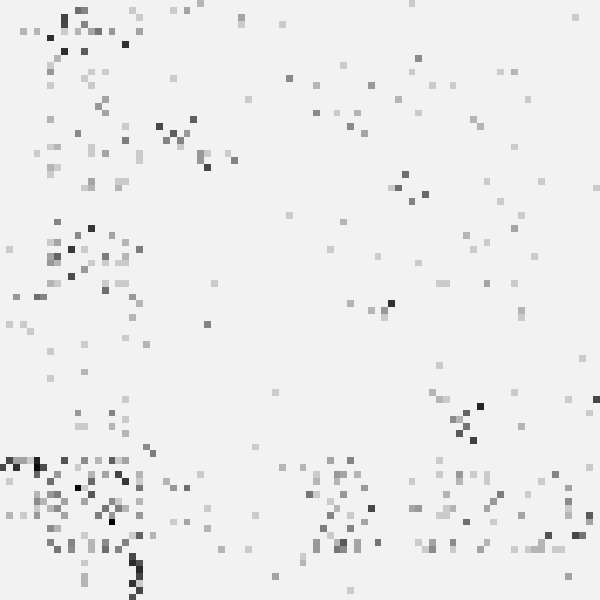
\includegraphics[scale=.25]{../figs/eckmann-small/parmat/observed}
\caption{Observed counts}
\end{subfigure}
~
\begin{subfigure}[b]{0.22\textwidth}
\centering
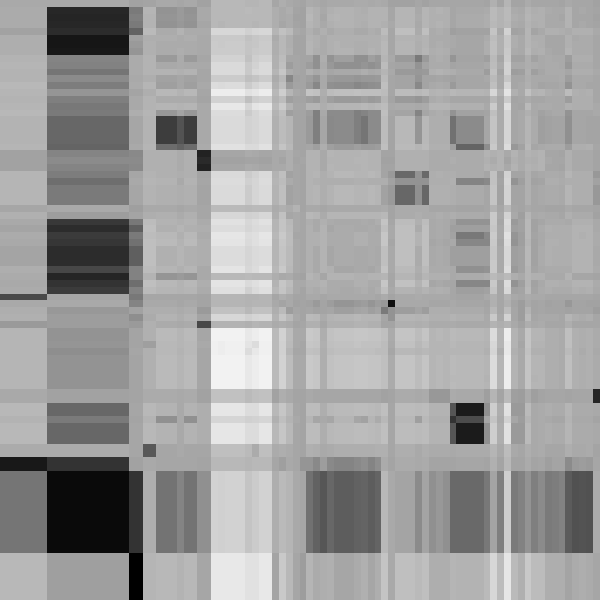
\includegraphics[scale=.25]{../figs/eckmann-small/parmat/1}
\caption{Intercept estimates}
\end{subfigure}
~
\begin{subfigure}[b]{0.22\textwidth}
\centering
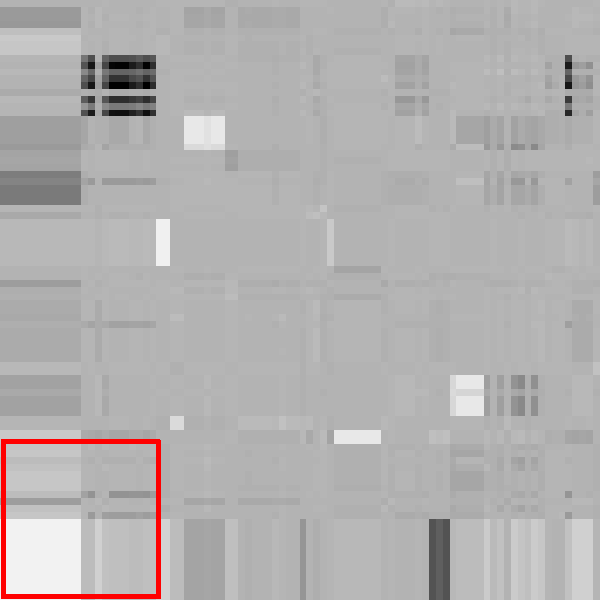
\includegraphics[scale=.25]{../figs/eckmann-small/parmat/2}
\caption{\texttt{ab-ba} estimates}
\end{subfigure}
~
\begin{subfigure}[b]{0.22\textwidth}
\centering
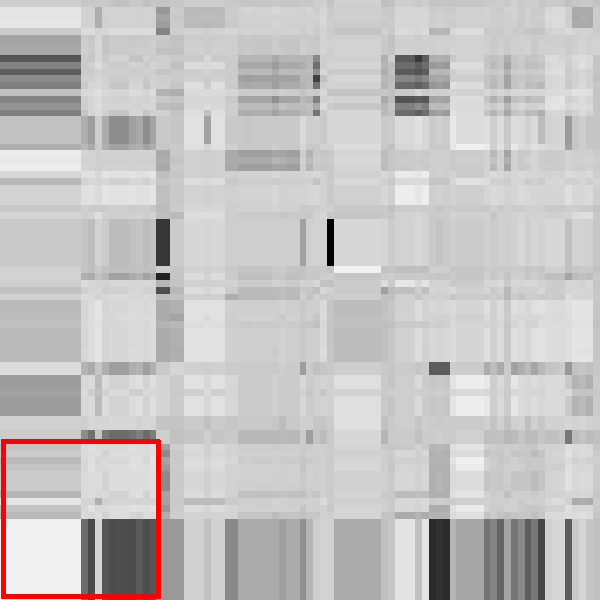
\includegraphics[scale=.25]{../figs/eckmann-small/parmat/3}
\caption{\texttt{ab-by} estimates}
\end{subfigure} \\
\begin{subfigure}[b]{0.22\textwidth}
\centering
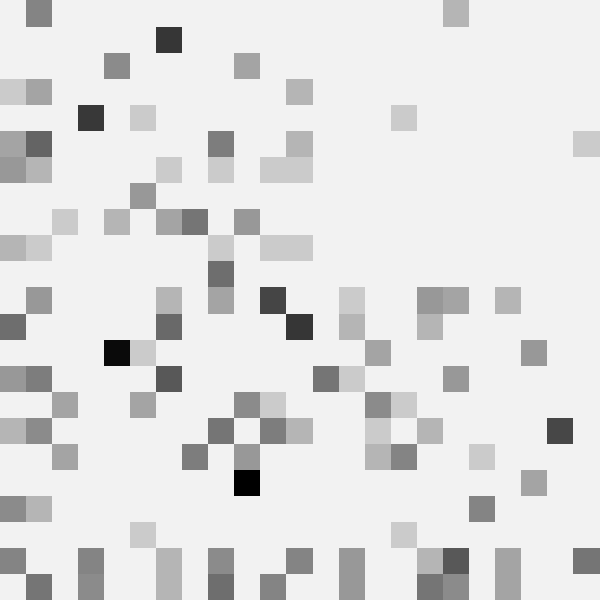
\includegraphics[scale=.25]{../figs/eckmann-small/parmat/observed-zoom}
\caption{Observed counts}
\end{subfigure}
~
\begin{subfigure}[b]{0.22\textwidth}
\end{subfigure}
\begin{subfigure}[b]{0.22\textwidth}
\centering
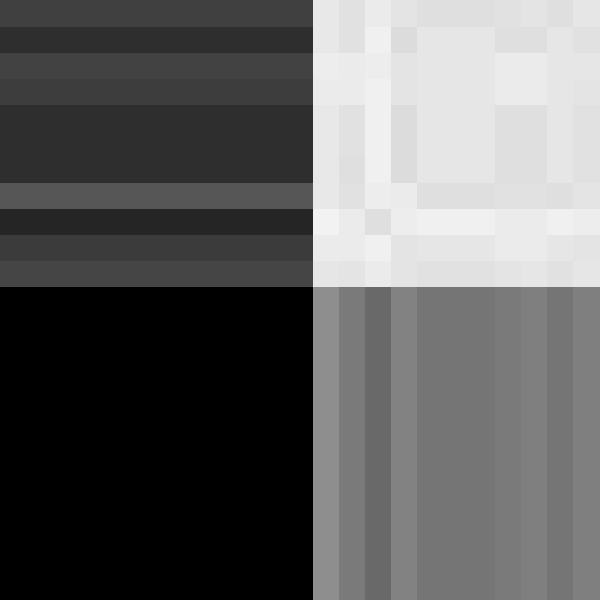
\includegraphics[scale=.25]{../figs/eckmann-small/parmat/1-zoom}
\caption{Intercept estimates}
\end{subfigure}
~
\begin{subfigure}[b]{0.22\textwidth}
\centering
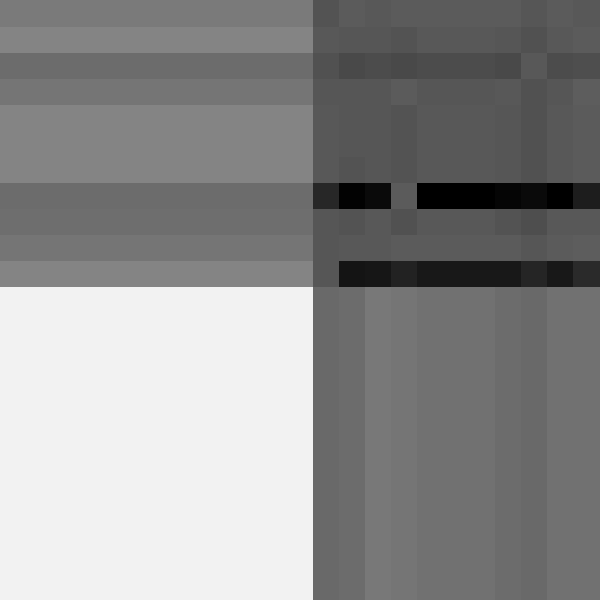
\includegraphics[scale=.25]{../figs/eckmann-small/parmat/2-zoom}
\caption{\texttt{ab-ba} estimates}
\end{subfigure}
\begin{subfigure}[b]{0.22\textwidth}
\centering
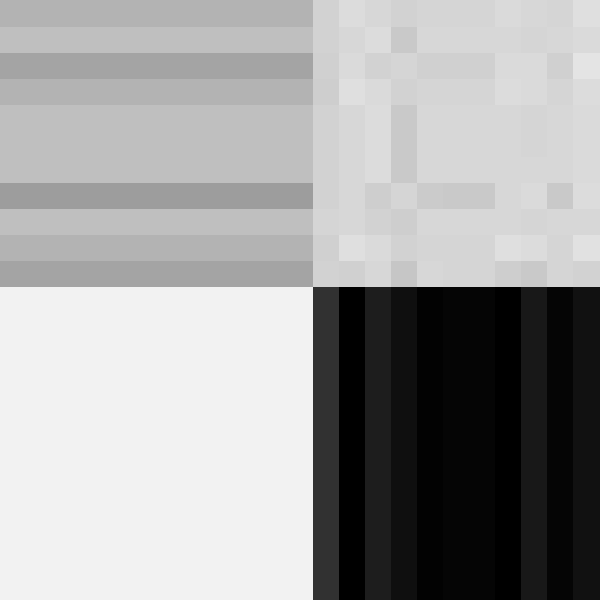
\includegraphics[scale=.25]{../figs/eckmann-small/parmat/3-zoom}
\caption{\texttt{ab-by} estimates}
\end{subfigure}
\caption{Comparing observed counts and parameter estimates.  Darker values are larger.  Estimates are rescaled posterior means $(\hat{\beta}_{z_i,z_j,p} - \hat{\mu}_p)/\hat{\sigma}_p$ for each dyad $(i,j)$.  Learned parameters suggest heterogeneity exists in both total activity (b) as well as dynamics, as seen in (c) and (d).  Figures (e-h) give a zoomed-in view of groups 1 and 3, showing that while the overall rate of (1,3) and (3,1) events is similar, the tendency for \texttt{ab-by} transitions differs.}
\label{fig:parmats}
\end{figure*}

We additionally perform experiments that evaluate the likelihood of future data under our model.   As our method jointly models \emph{which} dyads occur and \emph{when} they occur, any alternative method needs to also model these two aspects.  In this vein, we extend the above baselines by assuming each dyad is a Poisson process with estimated  rate $$\hat{\lambda}_{i,j}(t_m) = \frac{M}{t_M} \frac{r_{b}(i,j) + \xi}{\sum_{i,j} r_{b}(i,j) + \xi}$$, where $r_b(i,j)$ is the statistic for a given baseline (described above) and $\xi=1$ is a smoothing parameter.  
In Table ~\ref{tab:results} we compare the loglikelihood of held-out test data under our proposed model to each of these baselines.  In order to investigate the role of the number of clusters, we introduce an upper bound $K^*$ on the number of clusters during the fitting process.
Note that the model with $K^*=1$ is an important baseline -- it is simply a relational event model with no groups. There are a large number of other possible baselines that one might use, but most are not directly applicable to Table 2 as they do not work with events in continuous time.

For the synthetic data example introduced in Section \ref{sec:simulation} the fitted models with $K>1$ have predictive performance comparable to the true model; a standard relational event model does not perform as well because it does not have the flexibility to model the dynamics of each block separately.  For the classroom data set we see only a slight improvement with $K>1$, while with the mobile phone calls the $K=3$ model performs best.

In Table~\ref{tab:recall20} we include the corresponding results for the recall experiment at a cutoff of 5 and 20, respectively.  The results there are similar. As an example, using the Mobile data we are making a prediction of the next event among $89^2$ possible events: e.g., the next event is among the 5 highest-ranked edges 16.3 percent of the time by the $K*$=2 model. This is 1291 times more often than predicting events with our uniform baseline. Note that the absolute numbers for the baselines (e.g., zero in the 1st 3 decimal places for uniform) are so low because of the very large number of outcomes (e.g, $89^2$). For ranking, relative to all baselines including $K^*$=1, on the synthetic data set and Enron there are small systematic improvements, while on the phone and University data there are large systematic improvements.   Note that we used ranking performance (Table 3) to investigate the predictive power of the proposed models, as a function of $K^*$, rather than only evaluating test log-likelihood; the latter is what the model was optimized for and thus the optimal $K^*$ for Tables 2 and 3 need not agree.

\section{Discussion}


We have here introduced a family of relational event models that can flexibly capture heterogeneity in the underlying interaction dynamics.
Our approach generalizes traditional, static notions of stochastic equivalence on nodes (such as stochastic blockmodels) to the dynamic context. 
The proposed model family posits the existence of groups of nodes, such that all members of a group are governed by the same dynamic process, and groups are differentiated by having different dynamic processes. 
%PS: sentence below is incomplete (after the first "the")�..I decided to take it out anyway..
% Given a specification for the, the proposed method employs latent variables to model the heterogeneity in the event dynamics.
%is analogous to recent hierarchical extensions for latent position models \cite{Handcock2007} and exponential random graph models \cite{Schweinberger2011}.
%The method combines a latent variable framework (stochastic blockmodels) with a local dependence model for event sequences (relational event models \cite{Butts2008}).
%This provides detailed models of event dynamics among subsets of nodes while allowing for heterogeneity in the dynamics of the network as a whole.

%This analysis suggests 
Our approach has the ability to uncover systematic differences in dynamic behaviors among subsets of nodes, even in the absence of differences in marginal interaction rates.
% across a variety of data sets.
The analyses of Section \ref{sec:experiments} show that this model family has improved predictive accuracy over baseline methods on real data with respect to ranking tasks and the likelihood of unobserved data.
In particular, our proposed approach leads to improved predictive accuracy when compared to both (a) relational event models that lack latent clusters, and (b) stochastic blockmodels for count data, both of which are special cases of our model family.
Though prediction is not the main focus of our effort, these results provide evidence that having latent structure (i.e. $K > 1$) can lead to improvements in predictive power. However, our prediction results also show that it is easy to overfit with this model family. 
%If we restrict to K=2 on these small data sets, we systematically outperform the K=1 model. 
%{\red (TODO: confirm this)}
 As $K$ increases beyond 2 (e.g., for the unrestrained CRP prior), these models are prone to overfit. 
This is not surprising, given that the number of fitted parameters scales as the square of the number of components $K$ in the model. A natural direction worth exploring for this family is a class of priors that are more resistant to overfitting (e.g., by imposing more structure on the parameters within each group).
%  {\color{red} The choice of hierarchical structure would depend on the problem of interest, but such an approach could be of use when modeling multiple sequences simultaneously \cite{Arxiv?}.}

Another direction to explore is that of including different statistics in the specification of $\mathbf{s}(t,i,j,\mathcal{A}_t)$, modifying on the prior on each block's $\beta$ that induces some sparsity in the parameter estimates, and using our approach to study how the roles of these statistics vary across nodes.  
One potentially interesting extension, analogous to \cite{Airoldi2008}, would be to allow the latent class $z_i$ to be drawn from node-specific membership vectors $\pi_i$  after each change point.  Allowing underlying dynamics to be governed by a latent membership structure opens the door to a wide range of possibilities, with many opportunities for further elaboration.

%Other theories could be explored by including relevant statistics in the specification of $\mathbf{s}(t,i,j,\mathcal{A}_t)$, and similarly one can use our method to study how the roles of these statistics vary across nodes.  
%One interesting extension, analogous to \cite{Airoldi2008}, would allow the latent class $z_i$ to be drawn from node-specific membership vectors $\pi_i$  after each change point.  We leave this to future work.
%Alternatively, if nodes change groups.
%In some contexts such extensions might be substantively important and warrant future work.

%Our method learns about event dynamics within latent groups of individuals, but other types of heterogeneity likely exist in some data sets.  
%For example, dynamics might change over time \cite{Vu2011}.

%\subsubsection*{Acknowledgements}

\clearpage
\bibliographystyle{unsrt}
\bibliography{refs}
\end{document}
